\label{standard-call}
\subsubsection{Purpose}

Any subscribed passenger shall be able to request a taxi either through the web application or the mobile app.
After the request, the passenger is informed by the system about the waiting time and the code of the incoming taxi.

Requests shall be forwarded to available and active taxi drivers in the same zone of the passengers. Taxi drivers shall be able to accept or reject an incoming request.

\subsubsection{Response sequence}
\begin{figure}[h]
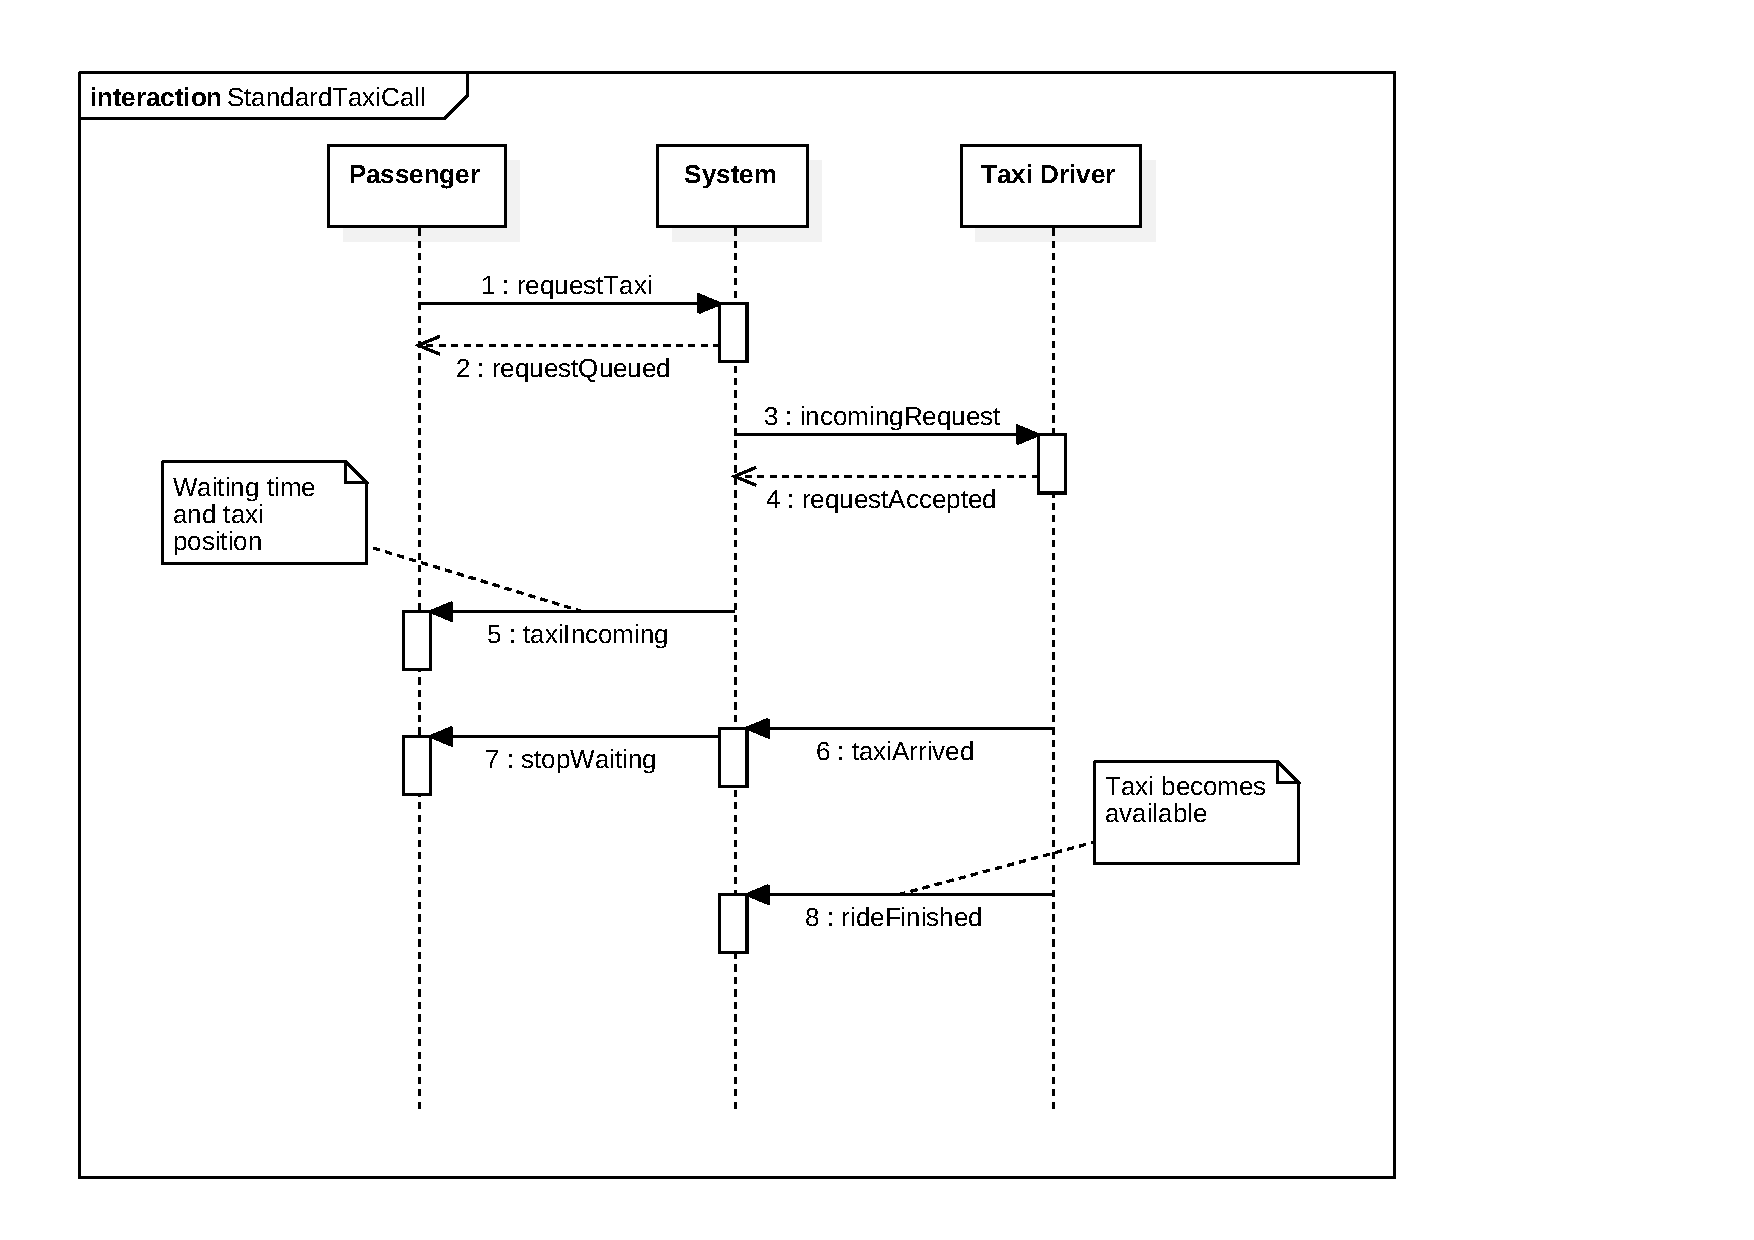
\includegraphics[width=\textwidth]{diagrams/sequence_taxicall.pdf}
\caption{Sequence diagram of a successful taxi call.}
\end{figure}

\subsubsection{Associated functional requirements}
\begin{enumerate}
\item The system must localize the passenger before he or she makes a taxi request.
\begin{enumerate}
\item (App) If GPS info is available and the passenger can be tracked within a radius of 50 m, then the passenger is presented with the option of using the current GPS position.
\item (App) If GPS info is not available or the precision is less than 50 m, then the app requests the passenger to insert a valid address. Then the address is shown on a map and the passenger can confirm its position.
\item (Web) In the web application the user is always requested to insert a valid address. Then the address is shown on a map and the user can confirm its position.
\end{enumerate}

\item When the system knows the passenger's position, it presents the passenger the option to request a taxi.
\item The system must ask the passenger for confirmation before delivering the taxi request.
\item After the passenger's confirmation of a taxi request, the request is delivered to the first taxi in the queue for the taxi zone in which the user is located.
\item Taxi requests are forwarded only to active taxi drivers which are located in the same taxi zone, who are not currently busy.
\item Taxi requests are processed in order of arrival.
\item When a taxi driver receives a request, the mobile application shows a notification and emits a sound.
\item When receiving a request, the taxi driver is presented with the possibility of accepting or denying it.
\item After having accepted a request, the taxi driver is automatically marked as "busy".
\item After having accepted a request, the mobile application shows to the taxi driver a map with the location of the passenger, and automatically starts navigation instructions on the app preferred by the taxi driver (Google Maps, Waze, TomTom, etc.).
\item After the taxi request is accepted, the app shows the passenger a map with the current position of the incoming taxi.
\item After the taxi request is accepted, the passenger is informed about the ETA for the incoming taxi.
\item The ETA for the incoming taxi is fetched from the server every 90 s.
\item The ETA for the incoming taxi is computed by the system considering the distance from the taxi to the passenger and the current traffic conditions.
\item When the taxi is within 20 m from the passenger, the app asks the taxi driver to confirm that the passenger is aboard.
\item When the taxi driver confirms that the passenger is aboard, the taxi request is marked as fulfilled and the system stops to show the waiting time to the passenger.
\item The taxi driver is presented by the mobile application with the option to end the ride.
\item When the taxi driver ends the ride, he or she is marked as available and gets re-inserted in the taxi queue of the taxi zone where he or she is located.
\end{enumerate}